\section{Results}
\subsection{Test of the Voronoi tessellation}
Even though the Voronoi tessellation is performed in the 3D space, an example of implementation for two agents in the 2D plane is here presented in \autoref{fig:Voronoi_example} because it is more understandable. The communication ranges are $R_{c1}=2.2, R_{c2}=0.55$ and a coverage factor of $\kappa=3$ has been used.  Here three different cases are reported: A) agents with point dimensions and $s_{max}=0$ (i.e. analogous to the continuous time implementation of the algorithm) and perfect localizations, B) finite physical encumbrance $\delta_1=0.25$, $\delta_2=0.15$, finite space $s_{max,1}=1$, $s_{max,2}=0.35$ and perfect localization, C) finite physical encumbrance, finite velocity and uncertainty in localization $\sigma_{1}^1=\sigma_{2}^2=0.05^2 \text{\textit{I}}_3, \sigma_{1}^2=0.1^2 \text{\textit{I}}_3, \sigma_{2}^1=0 \text{\textit{I}}_3$.
\begin{figure}[htb]
\centering
    \includegraphics[width=0.7\columnwidth]{images/fig_Voronoi_example.eps}
    \caption{Example of the Voronoi tessellation for two agents in the plane. $\mathcal{V}_A$ is build considering only the position of the agents, $\mathcal{V}_B$ considers finite dimensions and velocities while $\mathcal{V}_C$ considers also the uncertainties.}
    \label{fig:Voronoi_example}
\end{figure}
In case A, agent \textit{1} sees \textit{2} inside its communication range and sets its cell limit at half their distance; chute \textit{2} does not see \textit{1} and so its cell becomes the whole circle with radius $R_{c2}$. In case B, agents \textit{1} and \textit{2} in one-time step can reach the limit of the cell, so they have to shrink their old cells of $\delta_1$ and $\delta_2$. The Voronoi limit of agent \textit{2} moves inside the encumbrance of the chute itself. In case C, on top of what already happened in case B, \textit{1} further shrinks its limits so that in the direction between \textit{1} and \textit{2} the limit goes above \textit{1}. Meanwhile, \textit{2} increases its encumbrance, reducing its Voronoi limit more than the dimension of the previous area, leading the final cell to be a point. In that final condition, \textit{1} cannot move towards while \textit{2}, while \textit{2} cannot move at all.

\subsection{Example of localization}\label{subsec:ex_localization}
\autoref{fig:fig_self_update} reports an example of the localization done by one agent on itself when the EKF uses the GPS measurement and the model (labelled \textit{measure}) or only the latter (labelled \textit{model}). In this specific example, nine agents fall from $[500, 500, 1000]$ toward $[0,0,0]$, with the inverse kinematic enabled and the probability of having the GPS measure equal to 50\%. The iterations when the initial free-falling period and the landing on the ground are highlighted with dashed lines.
\begin{figure}[h]
\centering
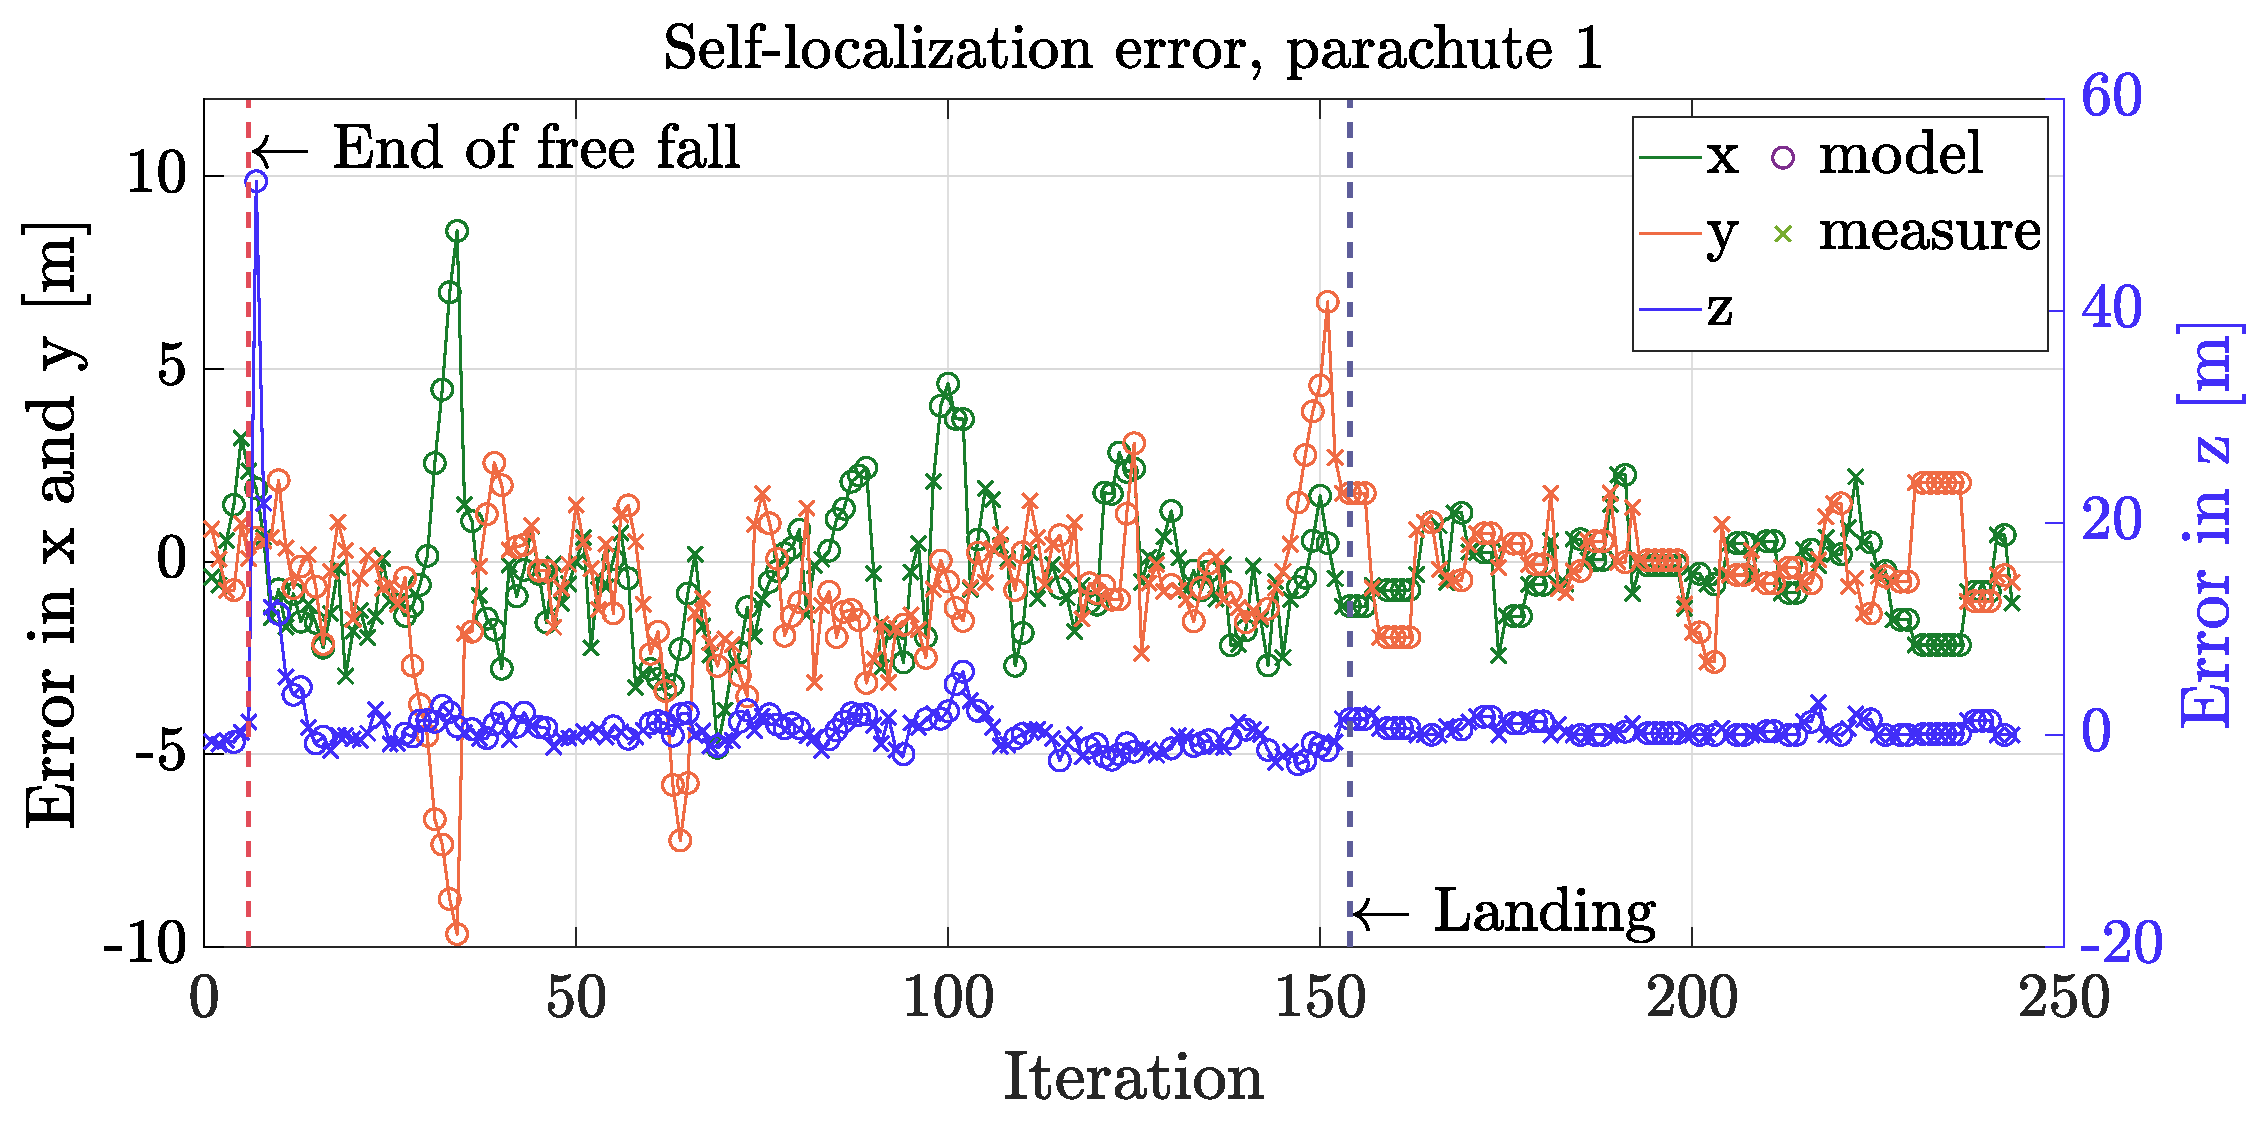
\includegraphics[width=\columnwidth]{images/fig_self_update.eps}
\caption{Error in the self-localization done by agent 1, with a probability of having the GPS measure of 50\%.}
\label{fig:fig_self_update}
\end{figure}
It could be seen that after the end of the free-falling part when the parachute opens and the falling velocity suddenly reduces, the localization error grows a lot, while it quickly decreases in a few iterations. It is also interesting to notice how there are no GPS measurements between iterations 27 and 34, so the error made by localizing with only the model grows. At iteration 35, a new GPS signal is available, and the error is reduced. Finally, the errors are lower after the landing because wind and input noises no longer affect the agent's position.
\subsection{Example of a complete swarm trajectory}\label{subsec:complete_sim}
\autoref{fig:3D_traj} shows the trajectory followed by 13 parachutes falling between the previous positions, while \autoref{fig:state} shows the time evolution of states and control inputs for one of the falling parachutes. The wind noise has been set to 3 $\left[\si{\meter\per\second}\right]$ in every direction.
\begin{figure}[h]
    \centering
    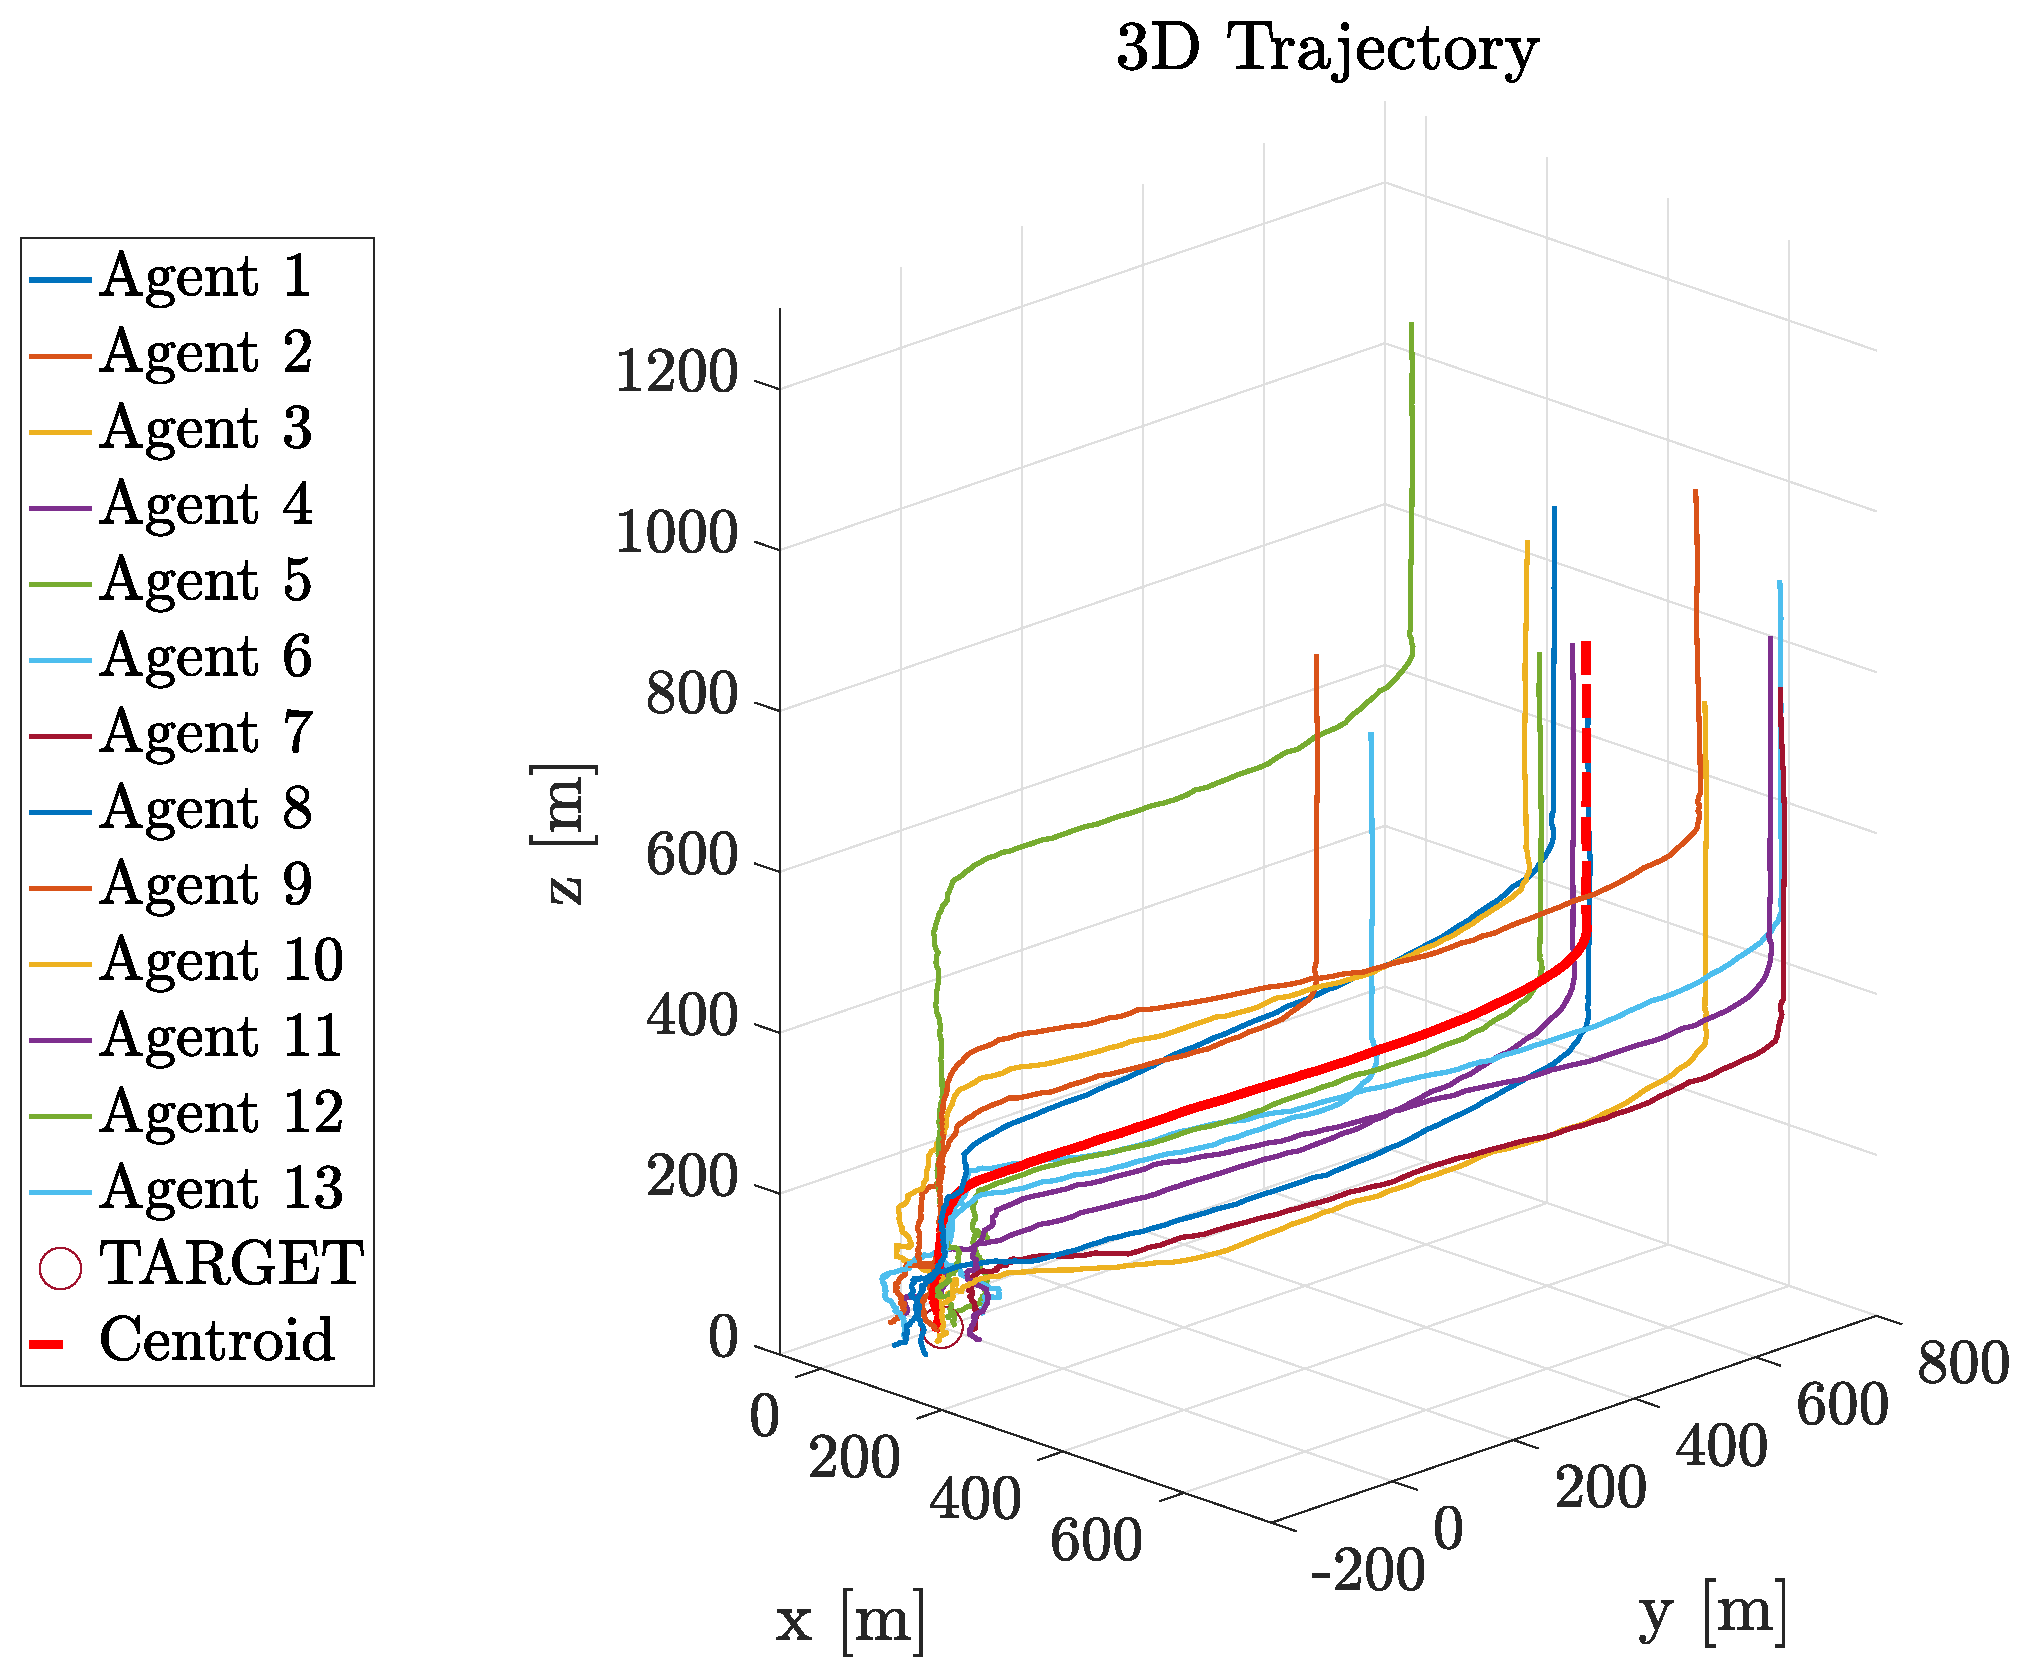
\includegraphics[width=\columnwidth]{images/fig_3D.eps}
    \caption{3D trajectory with 13 parachutes and all probabilities set to 1.}
    \label{fig:3D_traj}
\end{figure}
\begin{figure}[h]
    \centering
    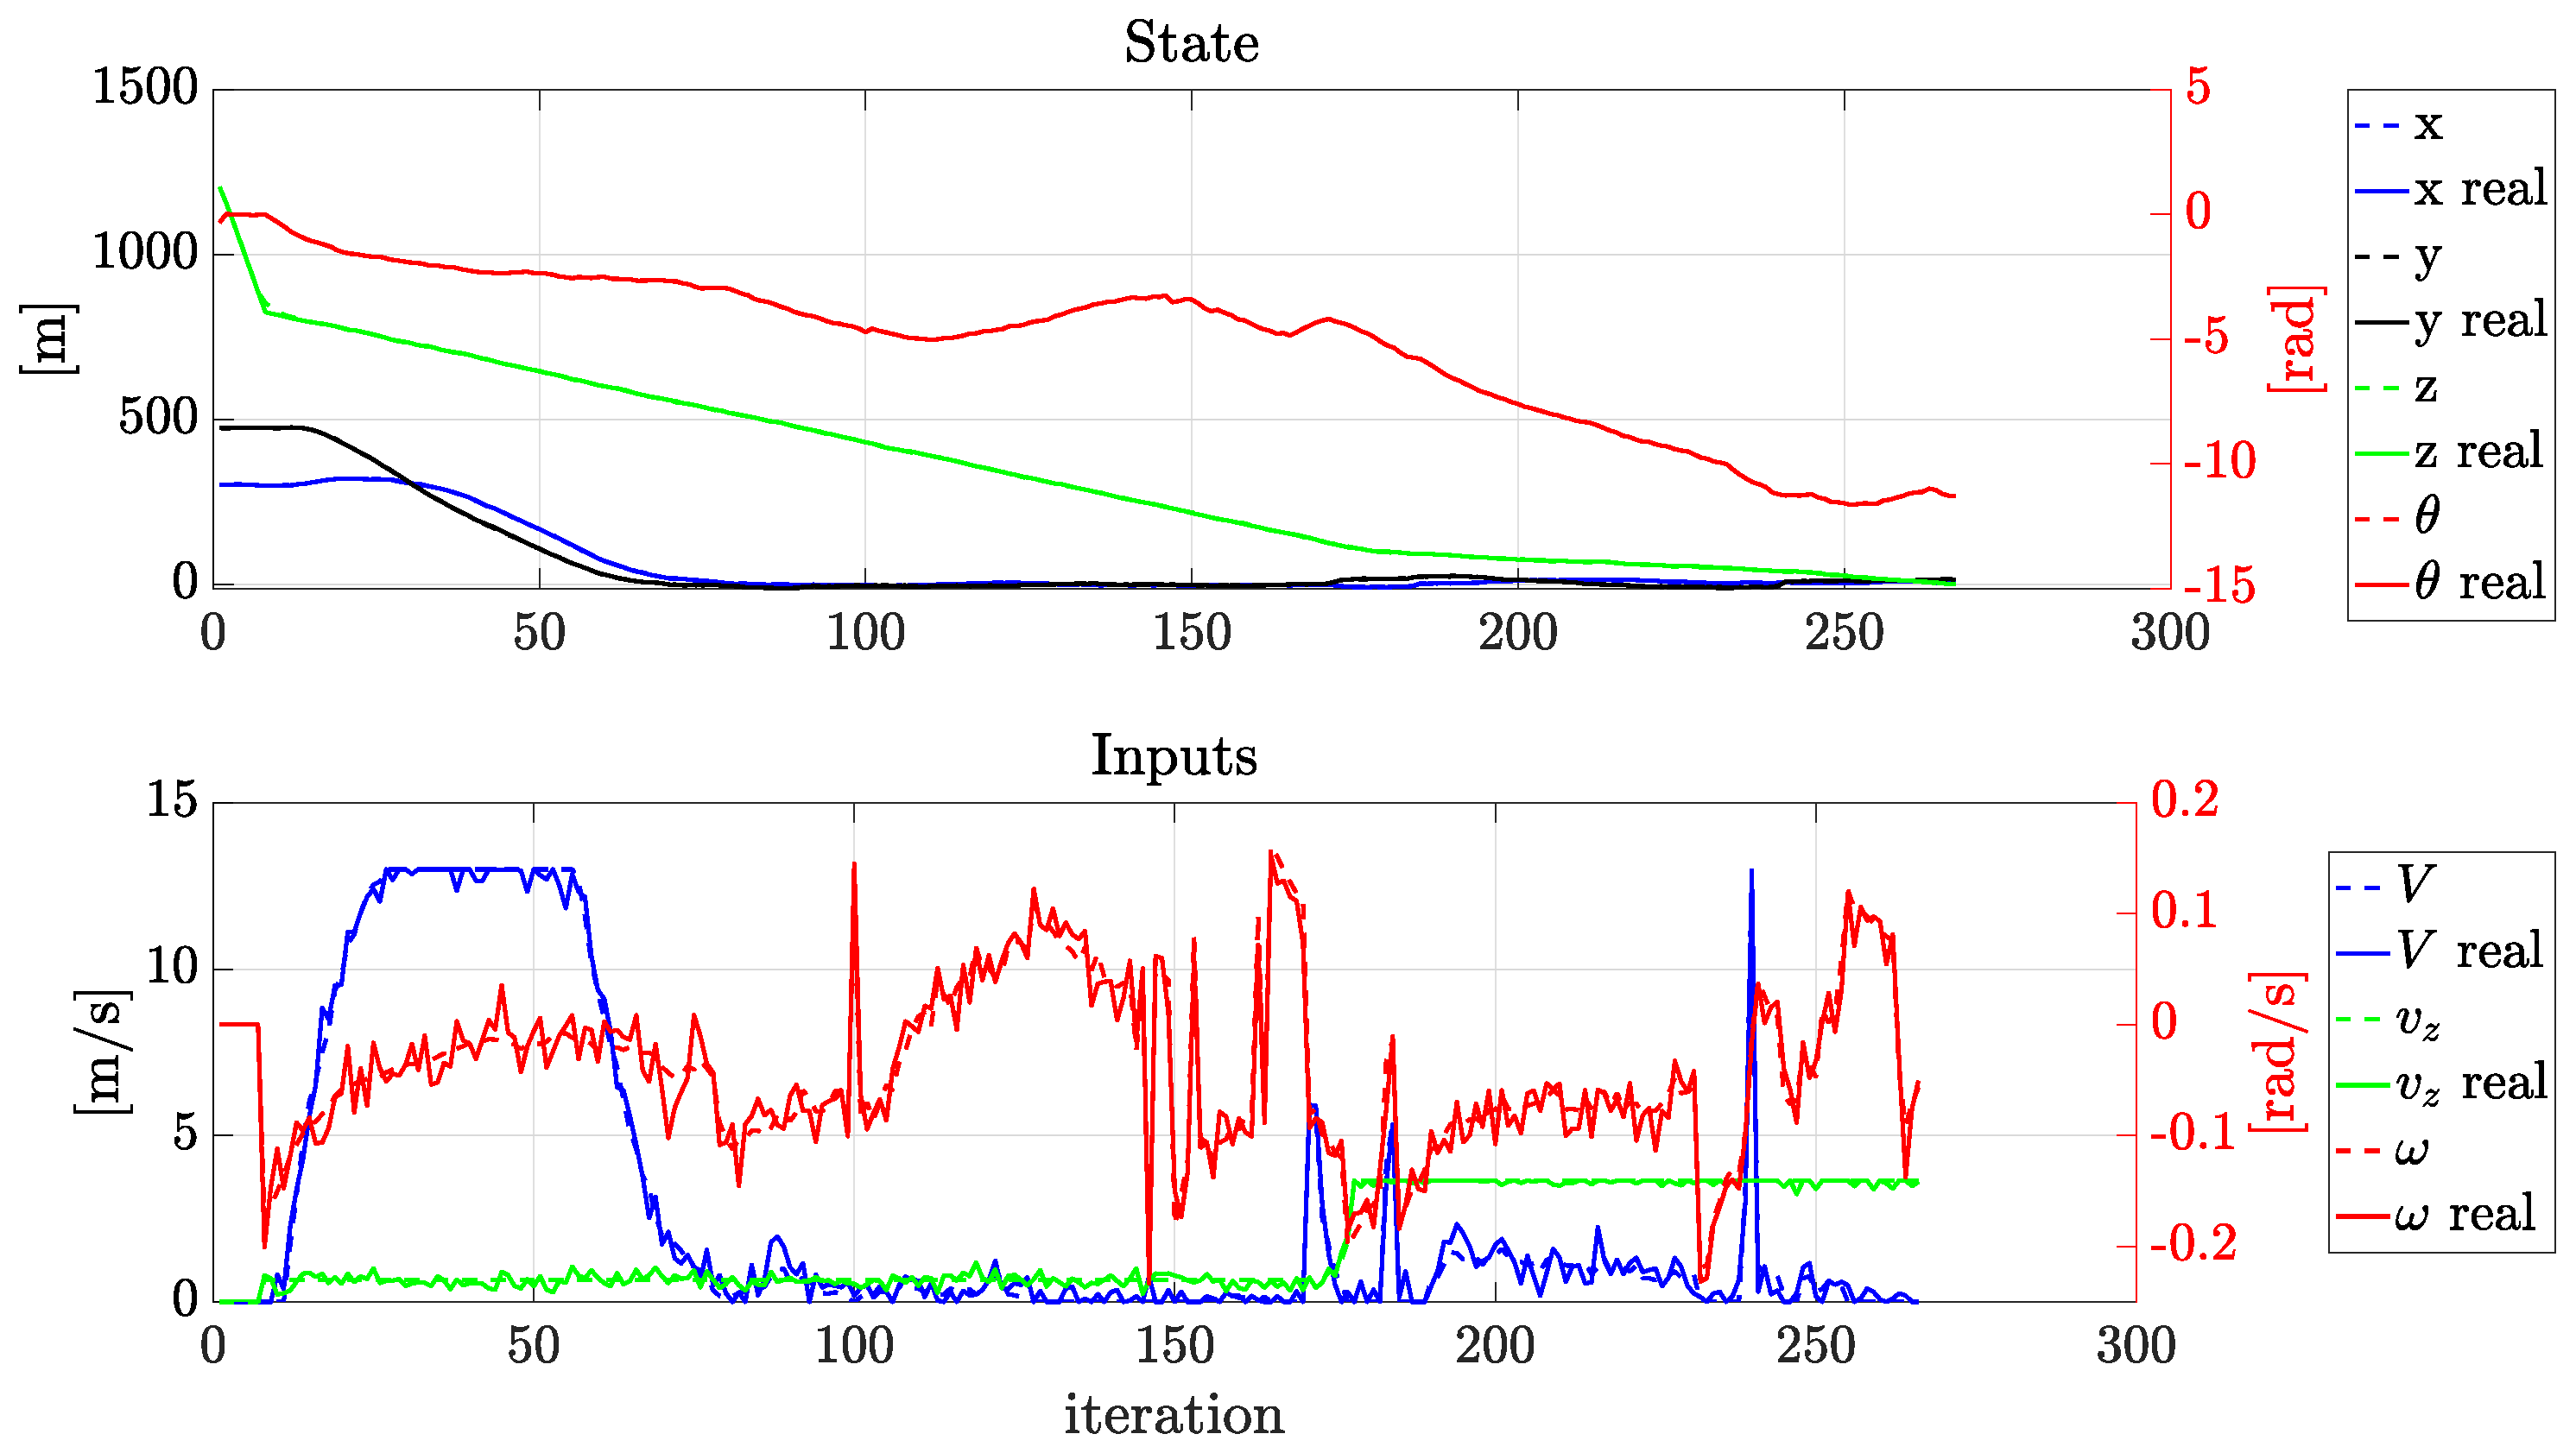
\includegraphics[width=\columnwidth]{images/fig_1.eps}
    \caption{States and inputs behaviour of agent 12.}
    \label{fig:state}
\end{figure}
It could be seen that the centroid (red dashed line of \autoref{fig:3D_traj}) reaches the target correctly, while the parachutes fall around it without any collision.\\
Regarding the inputs, it may be noticed that there is no actuation in the initial free-falling part. In contrast, in the final part, the control on the z-axis is saturated to reduce the speed before contact with the ground. Also, the forward velocity is saturated in the central part, where the agent moves toward the target. 

\subsection{Distributed WLS}
\autoref{fig:ab_IK} represents the standard deviation of the localization error committed by agent 7 of the simulation in \ref{subsec:ex_localization} in the localization of the others before and after distributing information via the WLS algorithm in the three directions. It must be noted that \textit{before WLS} considers the localization at the time steps when the relative distance measurement is performed or when the dynamic of the other is propagated through the model. On the other hand, \textit{after WLS} considers the result of the consensus algorithm, so in that instant, the localization can also be based only on the information shared by the network with the considered one.
\begin{figure}[h]
    \centering
    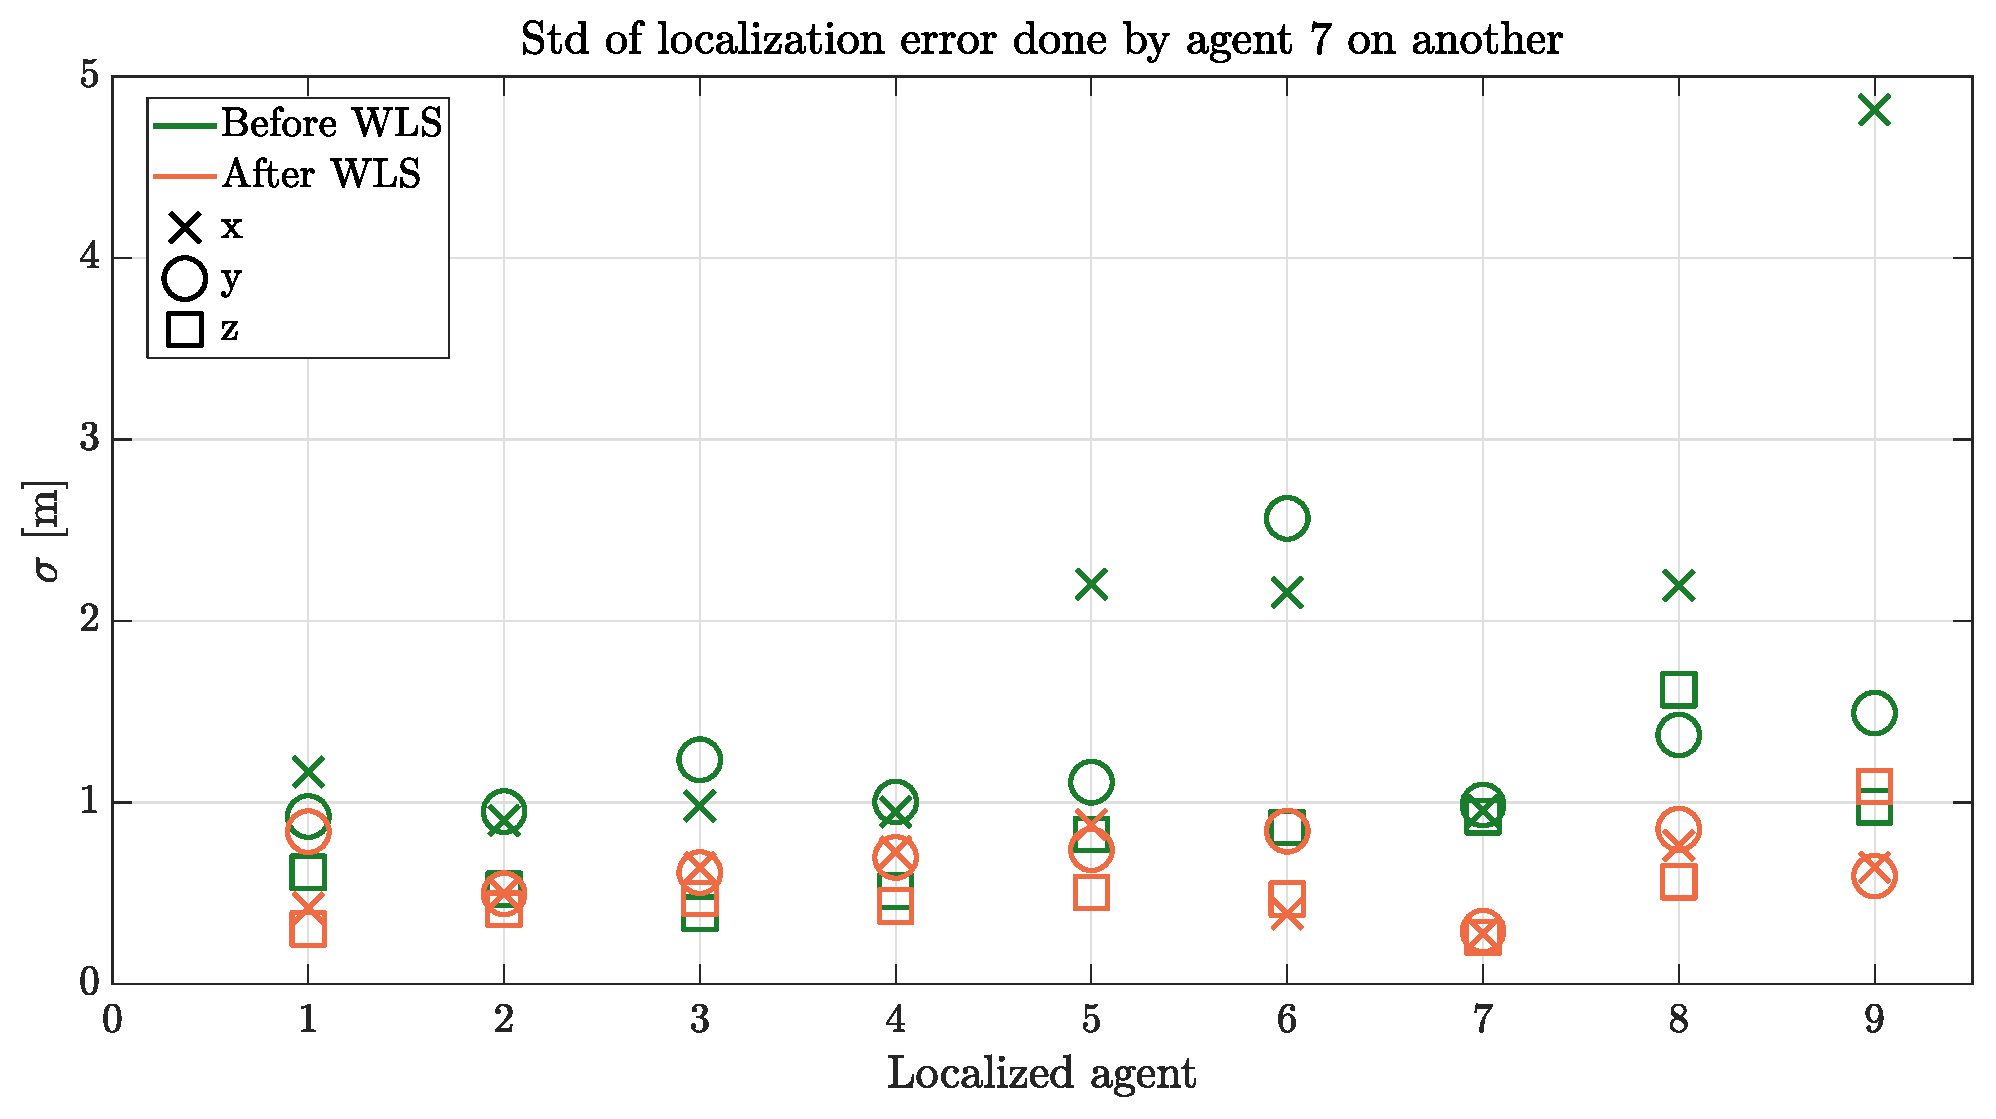
\includegraphics[width=\columnwidth]{images/mdl2_9chutes_be_wls.eps}
    \caption{Standard deviation of the error made by the parachute seven on the localization of the others.}
    \label{fig:ab_IK}
\end{figure}
Note that, as expected after the WLS, the error in the localization is reduced for all the agents.
\subsection{Effect of the Inverse Kinematics}
A comparative test has been done to test the IK's effectiveness in the navigation. In particular, several parachutes have been driven with and without using the IK. The initial conditions of the two cases are the same for a given round, and more rounds have been run. No uncertainties and noises have been introduced to highlight the effect of the navigation only. Finally, the distance between the centroid and the target has been computed alongside the agent's Root Mean Square (RMS) to the target distance. The mean results among multiple rounds are collected in \autoref{tab:IK_comparison}.
It could be seen that the IK approach reduces the dispersion of the chutes around the target, thanks to the postural task, for both models. In contrast, the distance of the global centroid from the target seems independent of the choice, except in the case of only one parachute. However, since having all the parachutes as near as possible to the target may be preferable, the RMS highlights the task's success.
\begin{table}[]
\scriptsize
  \caption{Comparison between the use of IK or not}
  \centering
  \begin{tabular}{ccccc|cccc}
  \hline
  & \multicolumn{4}{c}{Linear} & \multicolumn{4}{c}{Non-linear}\\
  \multicolumn{1}{c}{\#} & \multicolumn{2}{c}{Dist.} & \multicolumn{2}{c}{RMS} & \multicolumn{2}{c}{Dist.} & \multicolumn{2}{c}{RMS}\\
  \multicolumn{1}{l}{}  & IK & No IK & IK & No IK & IK & No IK & IK & No IK \\ \hline
  1   & 2.99 & 0.01 & 2.99 & 0.01 & 3.00 & 0.02 & 3.00 & 0.02  \\
  3   & 6.21 & 3.05 & 25.36 & 33.34 & 7.72 & 4.42 & 25.36 & 27.74 \\
  5   & 4.32 & 6.13 & 29.41 & 38.76 & 6.86 & 5.61 & 32.84 & 39.83 \\
  7   & 3.07 & 4.86 & 35.20 & 41.88 & 6.30 & 4.57 & 32.62 & 47.31 \\
  9   & 5.12 & 5.47 & 37.56 & 49.35 & 7.21 & 8.64 & 41.49 & 48.43 \\
  11  & 2.31 & 2.53 & 43.18 & 53.43 & 8.83 & 5.90 & 43.44 & 55.80 \\
  13  & 4.70 & 3.47 & 46.37 & 58.23 & 3.42 & 7.52 & 46.91 & 57.78 \\
  \hline
  \end{tabular}
  \label{tab:IK_comparison}
\end{table}



\subsection{Effect of the probabilities}
A parametric study has been conducted changing the probability of having the GPS or relative measurements between chutes, which simulates the ability of the real devices to acquire the data. This simulation considers nine parachutes of the nonlinear type affected by noise. The initial free-falling part and the final deceleration are turned off in the simulation because the localization takes some iterations to recover the error induced by the sudden change of vertical dynamics. In each test, one of the probabilities has been changed while the other has been kept constant at 100\%. After the simulation, the standard deviation of the localization error in the three directions has been computed for the self-localization in \autoref{fig:self_loc} and on the others in \autoref{fig:other_loc}. For the latter case, the mean of the error on all the others is reported.
\begin{figure}[h]
    \centering
    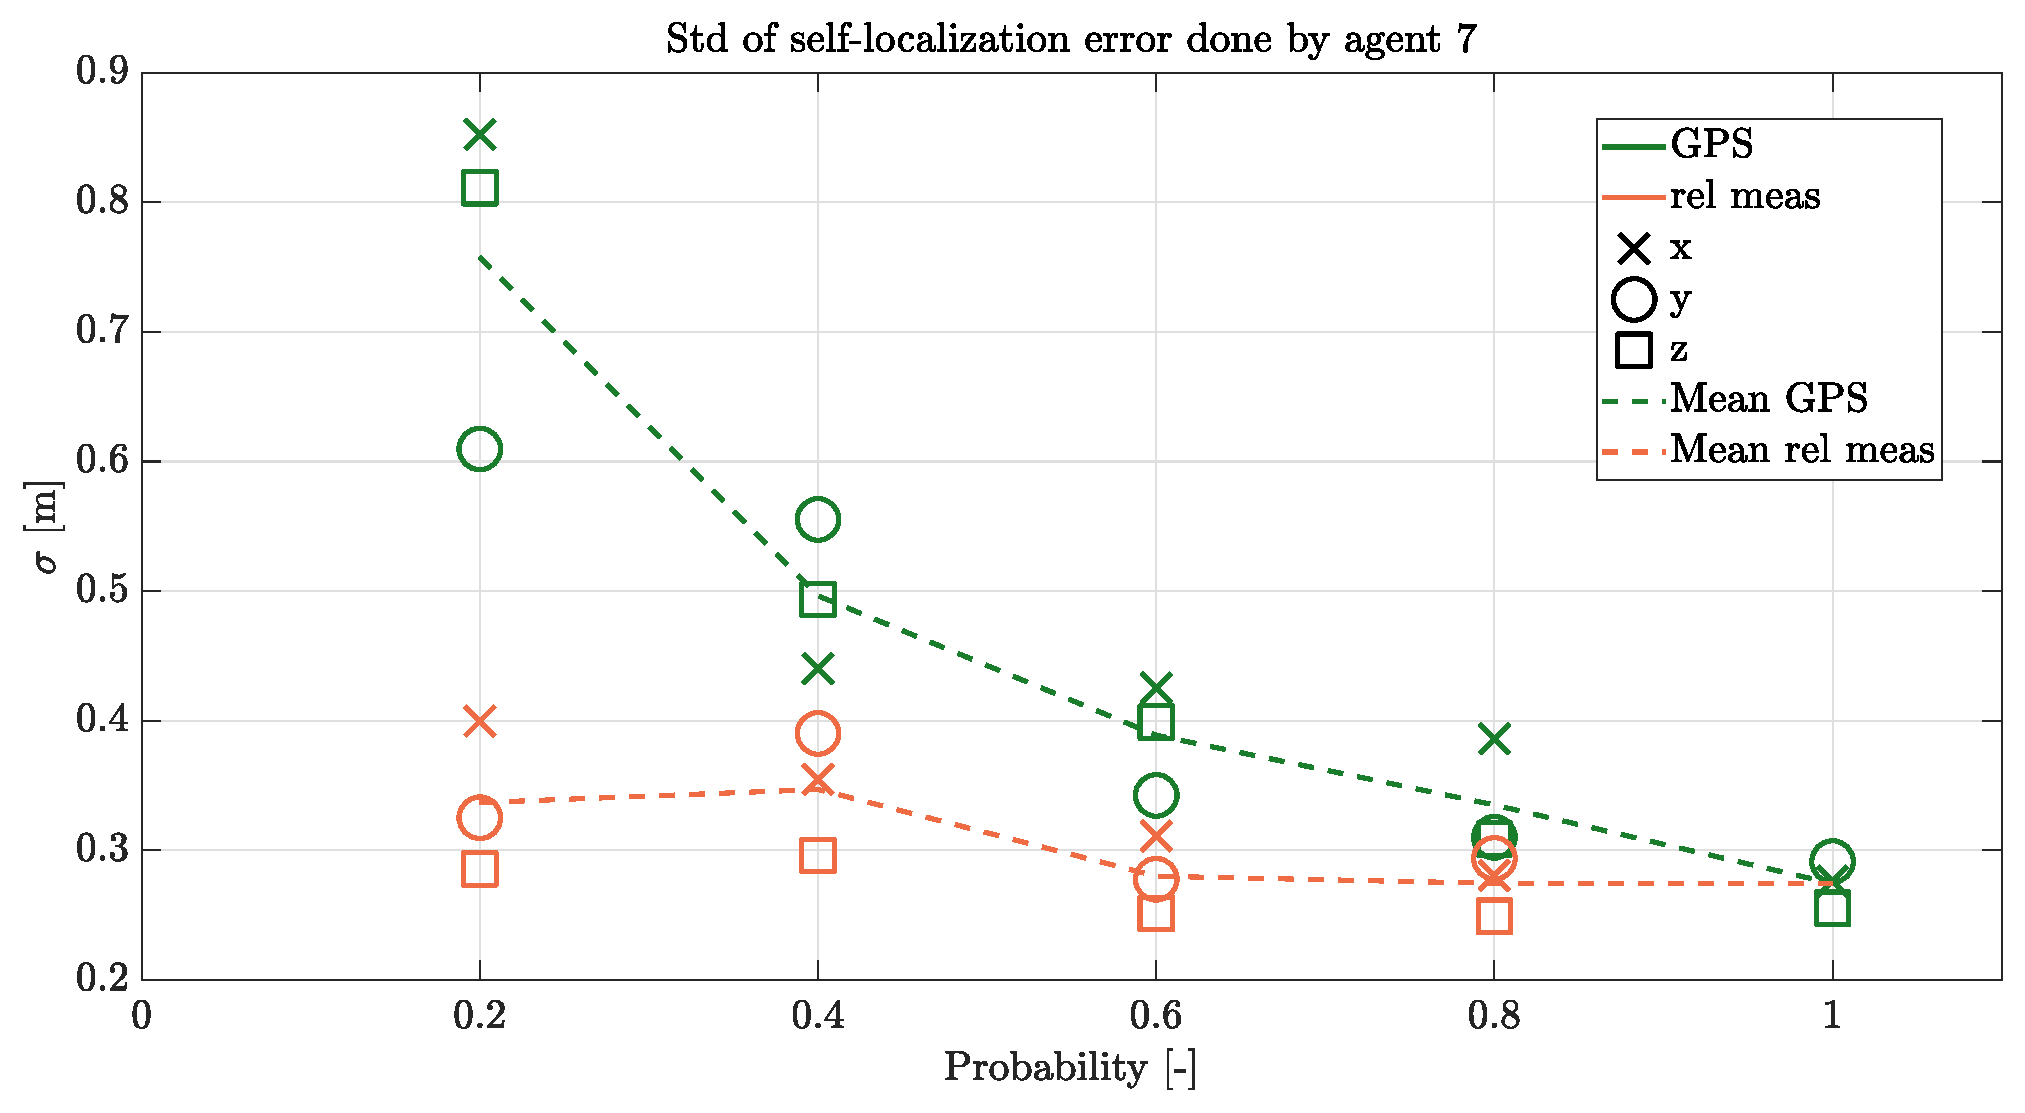
\includegraphics[width=\columnwidth]{images/mdl2_9chutes_parametric_beforeconsensus.eps}
    \caption{Standard deviation of the localization error made by the parachute seven on itself at different values of GPS and relative measurements probabilities.}
    \label{fig:self_loc}
\end{figure}
\begin{figure}[h]
    \centering
    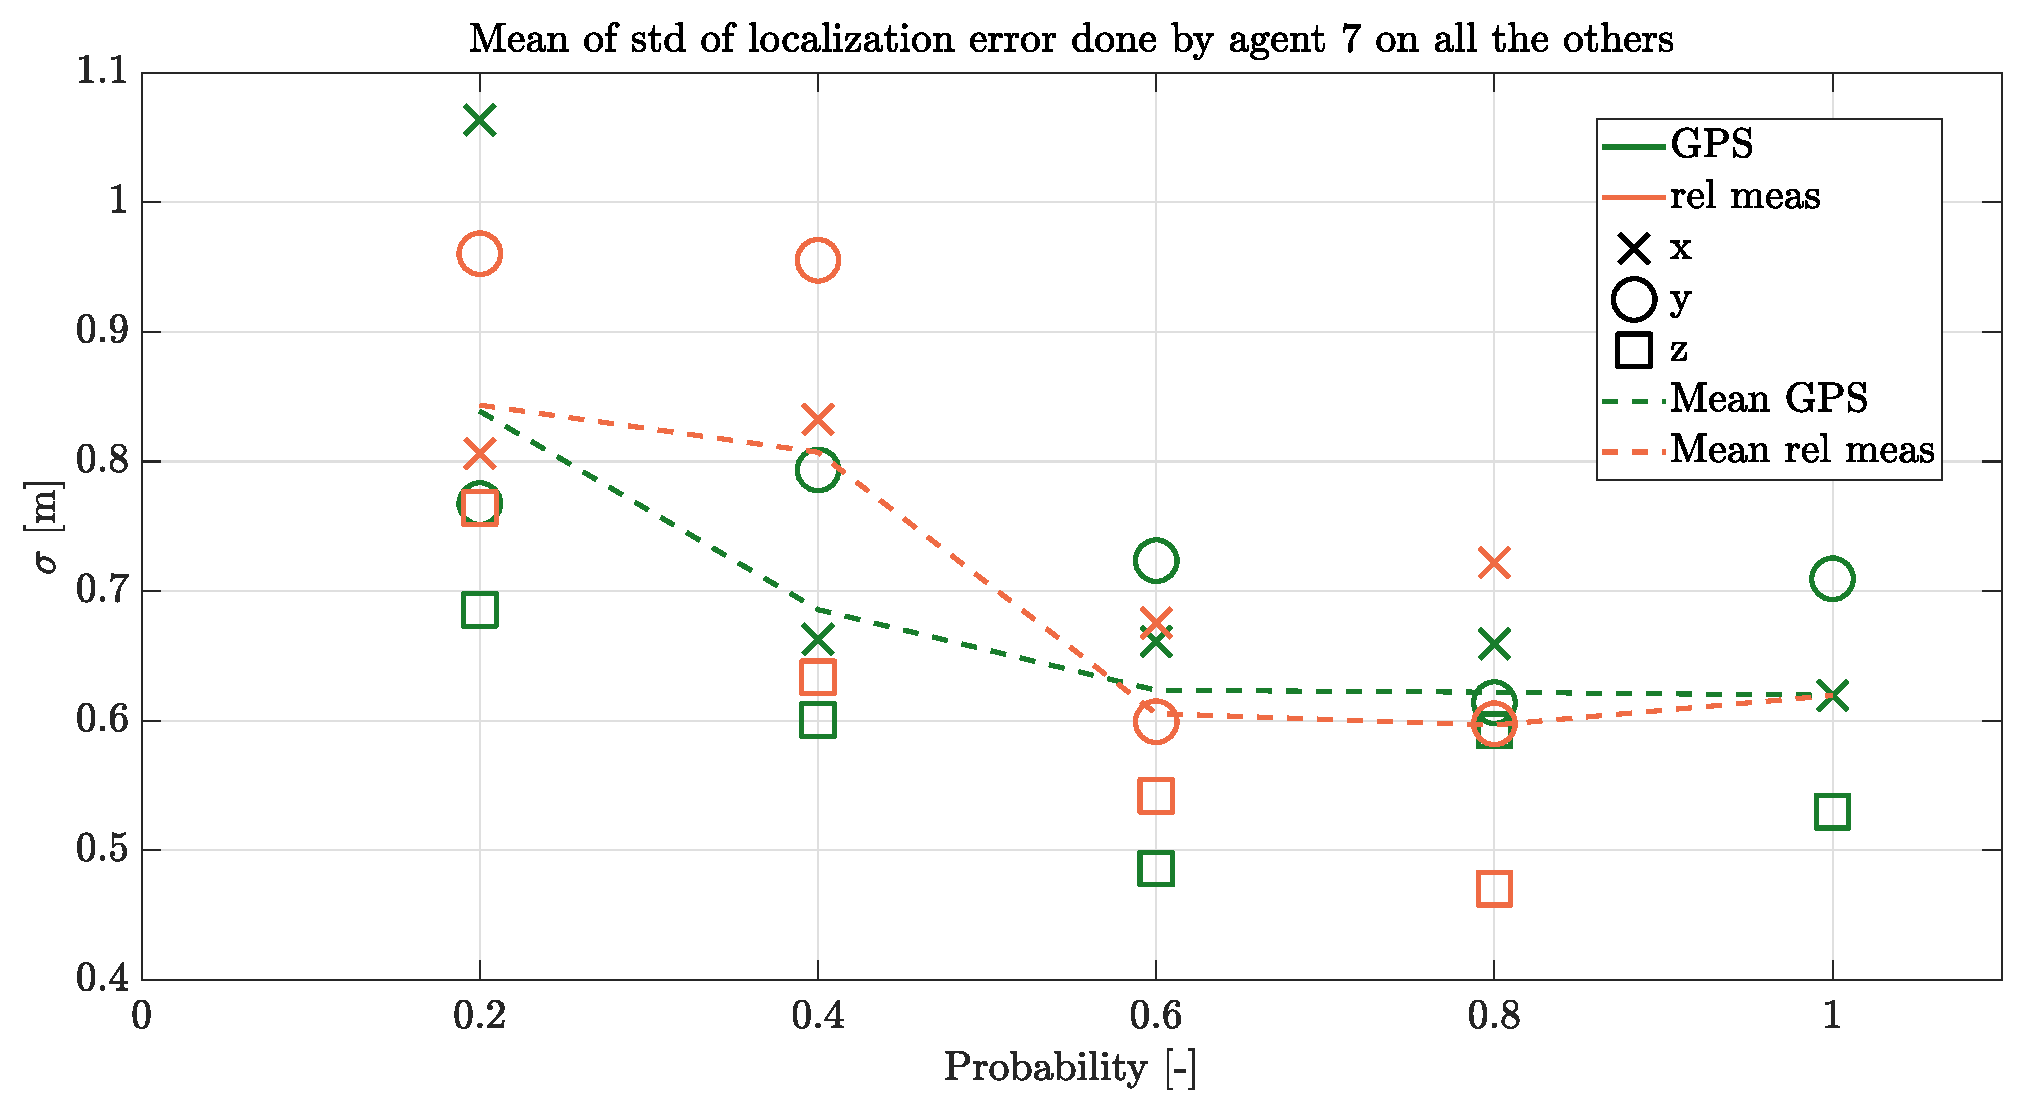
\includegraphics[width=\columnwidth]{images/mdl2_9chutes_parametric_loc_others.eps}
    \caption{Standard deviation of the localization error made by parachute seven on the other parachutes at different values of GPS and relative measurements probabilities.}
    \label{fig:other_loc}
\end{figure}
The graph shows that the GPS probability highly affects the self-localisation error, while it is less by the relative measurement. This may be due to two facts. The first is that the GPS alone can provide good localization, so the further information added by the relative measurement has a small contribution to the estimation. Furthermore, the probability of having the relative measurement is conditioned by the distance between agents, which in our simulation depends on its evolution.\\
On the other hand, the two effects are more combined in the localization errors made on the others since, for this analysis, the possibility of exchanging messages rules the process. In fact, when the agents are not close enough, they cannot exchange information with one another. Hence, the collected information (independently from its source) cannot be shared, and no contribution can be provided to the localization. Furthermore, when the connectivity is not always ensured, the effect of the error committed by propagating the states with the model is more significant.